\documentclass[a4paper,12pt]{article}

%%% Работа с русским языком
\usepackage{cmap}					% поиск в PDF
\usepackage{mathtext} 				% русские буквы в формулах
\usepackage[T2A]{fontenc}			% кодировка
\usepackage[utf8]{inputenc}			% кодировка исходного текста
\usepackage[english,russian]{babel}	% локализация и переносы
\usepackage{xcolor}
\usepackage{hyperref}
 % Цвета для гиперссылок
\definecolor{linkcolor}{HTML}{799B03} % цвет ссылок
\definecolor{urlcolor}{HTML}{799B03} % цвет гиперссылок

\hypersetup{pdfstartview=FitH,  linkcolor=linkcolor,urlcolor=urlcolor, colorlinks=true}

%%% Дополнительная работа с математикой
\usepackage{amsfonts,amssymb,amsthm,mathtools} % AMS
\usepackage{amsmath}
\usepackage{icomma} % "Умная" запятая: $0,2$ --- число, $0, 2$ --- перечисление

%% Номера формул
%\mathtoolsset{showonlyrefs=true} % Показывать номера только у тех формул, на которые есть \eqref{} в тексте.

%% Шрифты
\usepackage{euscript}	 % Шрифт Евклид
\usepackage{mathrsfs} % Красивый матшрифт

%% Свои команды
\DeclareMathOperator{\sgn}{\mathop{sgn}}

%% Перенос знаков в формулах (по Львовскому)
\newcommand*{\hm}[1]{#1\nobreak\discretionary{}
{\hbox{$\mathsurround=0pt #1$}}{}}
% графика
\usepackage{graphicx}
\graphicspath{{pictures/}}
\DeclareGraphicsExtensions{.pdf,.png,.jpg}
\author{Бурмашев Григорий, БПМИ-208}
\title{ТВиМС, дз -- 5}
\date{\today}
\begin{document}
\maketitle
\section*{Номер 1}
\begin{center}
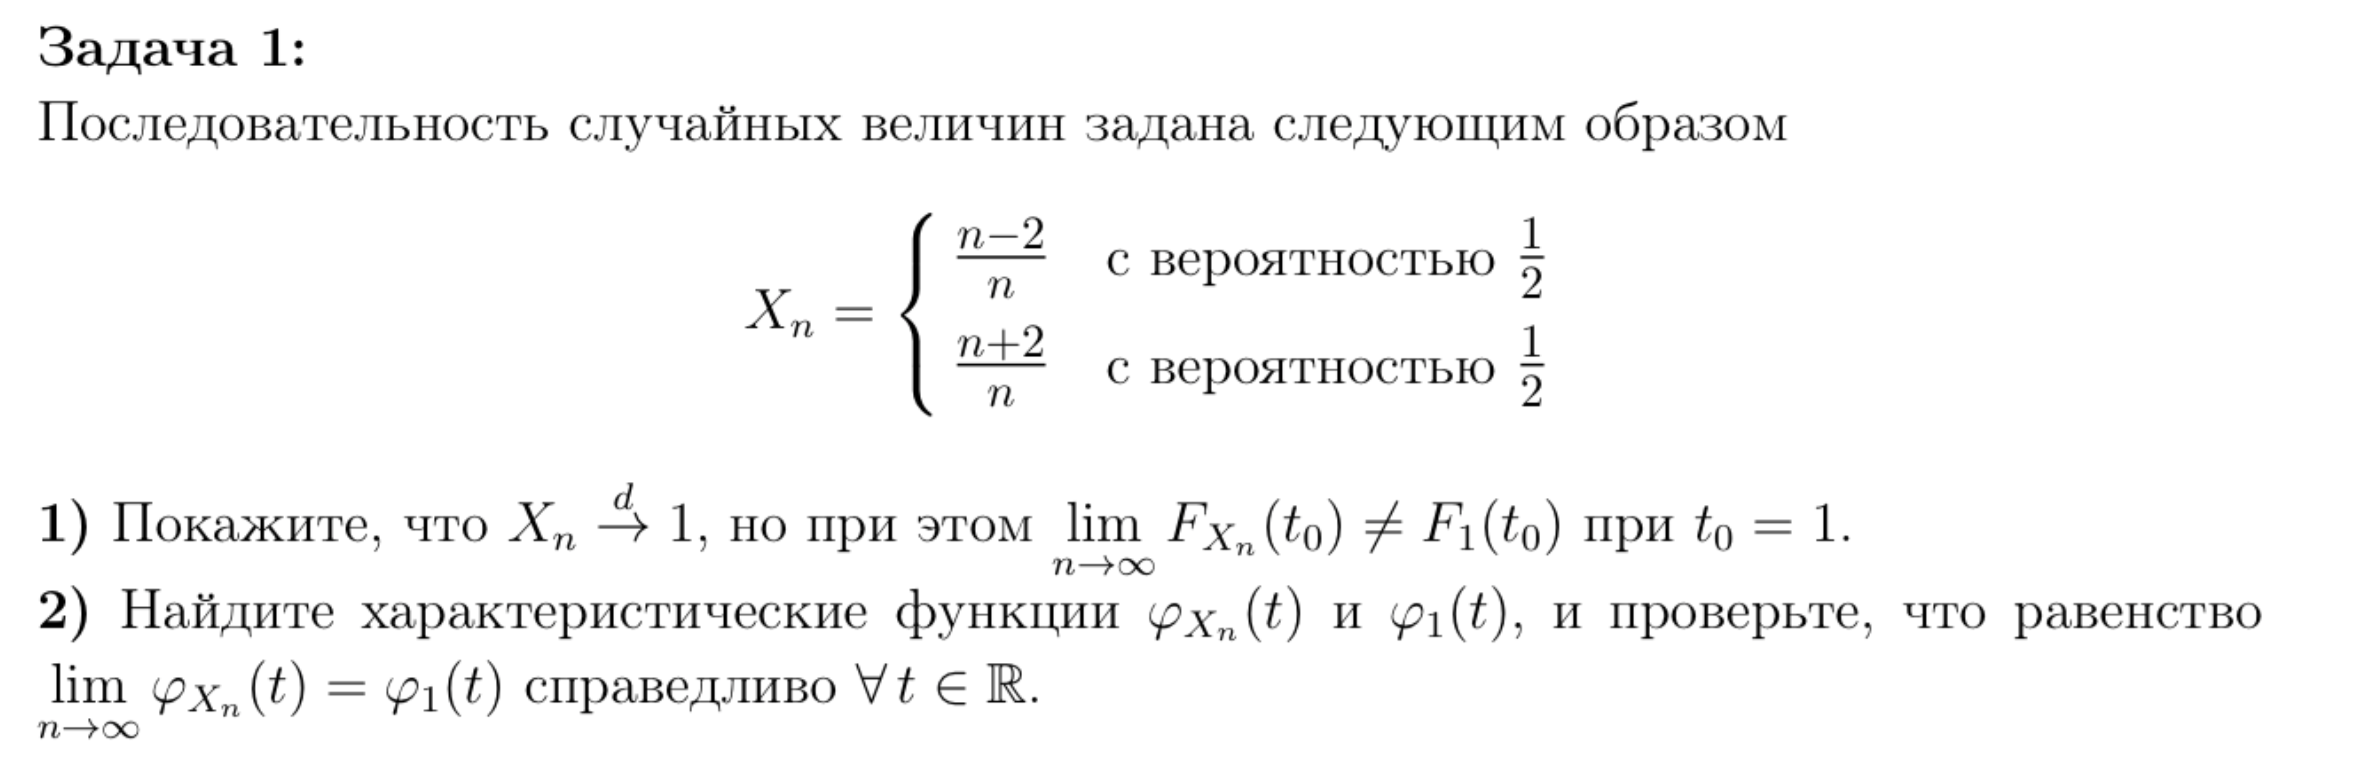
\includegraphics[scale=0.4]{1.png}
\end{center}
\subsection*{1)}
Посмотрим на функцию распределения для нашей последовательности:
\[
F_{X_n} (t) = 
\begin{cases}
0, &t < \frac{n-2}{n} \\
1, &t > \frac{n + 2}{n} \\
\frac{1}{2} &\text{ иначе, т.е когда внутри отрезка}
\end{cases}
\]
А для решения первого пункта посмотрим еще и на $F_1(t)$:
\[
F_1(t) = 
\begin{cases}
0, &t < 1 \\
1, &t \geq 1
\end{cases}
\]
Теперь проверим сходимость по распределению (по определению). Для этого устремим $n$ в бесконечность. Заметим, что при таких $n$ $ \frac{n - 2}{n} \rightarrow 1, \frac{n - 2}{n} \rightarrow 1$:
\[
\lim_{n \rightarrow \infty} F_{X_n} (t) = 
\begin{cases}
0, &t < 1 \\
1, &t \geq 1
\end{cases}
\]
Мы видим, что это в точности $F_1(t)$, т.е:
\[
\lim_{n \rightarrow \infty} F_{X_n}(t) = F_1(t)
\]
А значит:
\[
X_n \overset{d}{\longrightarrow} 1
\]
Теперь же посмотрим, что происходит в $t_0 = 1$ (это верно по определению $X_n$):
\[
\lim_{n \rightarrow \infty} F_{X_n}(t_0) = \lim_{n \rightarrow \infty} P(X_n \leq 1) = \lim_{n \rightarrow \infty} \frac{1}{2} = \frac{1}{2}
\]
В свою очередь для $F_1$:
\[
F_1(t_0) = P(1 \leq 1) = 1
\]
Мы видим, что в этой точке они не равны друг другу, т.е:
\[
\lim_{n \rightarrow \infty} F_{X_n}(t_0) \neq F_1(t_0), \;  t_0 = 1
\]
\begin{center}
\textbf{Ч.Т.Д} 
\end{center}
\subsection*{2)}
Хотим найти характеристические функции. Сначала для $X_n$. По определению:
\[
\varphi_{X_n}(t) = Ee^{itX_{n}}
\]
Распишем по определению $X_n$:
\[
Ee^{itX_{n}} = 
\frac{1}{2} \cdot e^{it \frac{n - 2}{n}} + \frac{1}{2} \cdot e^{it \frac{n + 2}{n}}
\]
А для $1$:
\[
\varphi_{1}(t) = Ee^{it1} = e^{it}
\]
Функции нашли, теперь посмотрим на предел, как я упоминал ранее, дроби из определения $X_n$ стремятся к единичке, а значит:
\[
\lim_{n \rightarrow \infty} \varphi_{X_n}(t) = \frac{1}{2}e^{it \cdot 1} + \frac{1}{2}e^{it \cdot 1} = e^{it} 
\]
Ну а это в точности $\varphi_1(t)$, причем при любых $t$, т.е:
\[
\lim_{n \rightarrow \infty} \varphi_{X_n}(t) = \varphi_1(t) \; \forall t \in \mathbb{R}
\]
\begin{center}
\textbf{Ч.Т.Д}
\end{center}
\clearpage
\section*{Номер 2}
\begin{center}
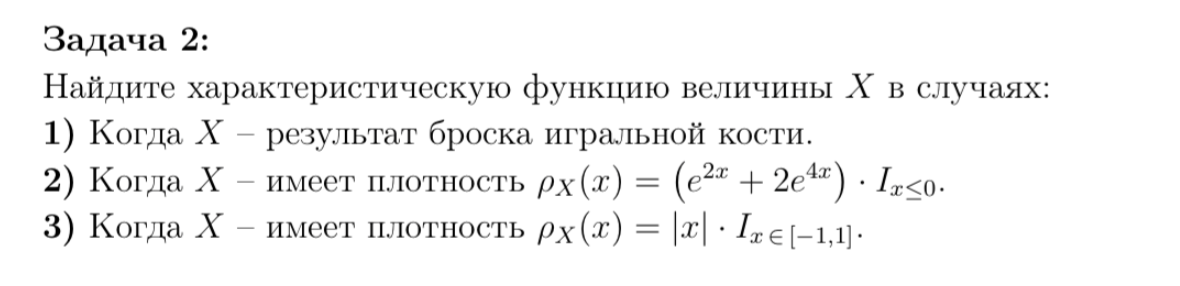
\includegraphics[scale=0.6]{2.png}
\end{center}
\subsection*{a)}
Пусть $X$ -- результат броска игральной кости. У кости 6 граней, вероятность выпадения каждой равна $\frac{1}{6}$, а значит можем расписать характеристическую функцию по определению:
\[
\varphi_X(t) = E\left(e^{itX}\right) = \frac{1}{6} \left(
e^{it}
+ e^{it2} 
+
\ldots
+ e^{it6}
\right)
\]
\begin{center}
\textbf{Ответ: } 
\[
\varphi_X(t)  = \frac{1}{6} \left(
e^{it}
+ e^{it2} 
+
\ldots
+ e^{it6}
\right)
\]
\end{center}
\subsection*{b)}
\[
\rho_X(x) = (e^{2x} + 2e^{4x}) \cdot I_{x \leq 0}
\]
Собственно расписываем по определению:
\[
\varphi_X(t) = E \left( e^{itX} \right) =
\int\limits_{-\infty}^{+\infty} e^{itx} \rho_x(x) dx (=)
\]
Теперь расписываем плотность с учетом индикатора
\[
(=) 
\int\limits_{-\infty}^{0} e^{itx}(e^{2x} + 2e^{4x})) dx  + 0 = 
\int\limits_{-\infty}^0 
\left(
e^{itx + 2x} + 2e^{itx + 4x} \right) dx
=
\]
\[
=
\int\limits_{-\infty}^0 
e^{itx + 2x} dx
+
\int\limits_{-\infty}^0 
2e^{itx + 4x} dx
=
\frac{e^{(2 + it)x}}{2 + it} \Bigg|_{-\infty}^0 +\frac{2e^{(4 + it)x}}{4 + it} \Bigg|_{-\infty}^0 
=
\frac{1}{it + 2} + \frac{2}{it + 4} - 0 - 0 = \frac{1}{it + 2} + \frac{2}{it + 4}
\]
\begin{center}
\textbf{Ответ: } 
\[
 \frac{1}{it + 2} + \frac{2}{it + 4}
\]
\end{center}

\subsection*{c)}
\[
\rho_X(x) = |x|  \cdot I_{x \in [-1, 1]}
\]
Собственно расписываем по определению:
\[
\varphi_X(t) =\int\limits_{-\infty}^{+\infty} e^{itx} \rho_x(x) dx = -\int\limits_{-1}^0 e^{itx} x dx + \int\limits_0^1 e^{itx} x dx (=)
\]
Найдем этот интеграл:
\[
\int e^{itx} x dx \overset{\text{и.п.ч}}{=}
\begin{bmatrix}
u = x \\
du = 1 \\
dv = e^{itx} \\
v = \frac{e^{itx}}{it}
\end{bmatrix}
=
 \frac{e^{itx}}{it} x - \int\frac{e^{itx}}{it} dx =  \frac{e^{itx}}{it} x  + \frac{e^{itx}}{i^2t^2} =\frac{e^{itx}}{it} x  + \frac{e^{itx}}{t^2} 
\]
Подставляем:
\[
(=) -\left( \frac{e^{itx}}{it} x  + \frac{e^{itx}}{t^2} \right)  \Bigg|_{-1}^0 + \left( \frac{e^{itx}}{it} x  + \frac{e^{itx}}{t^2} \right)  \Bigg|_0^1  = 
\]
\[
=
- \left(
\frac{1}{t^2}
- \left(
-
\frac{e^{-it}}{it} + \frac{e^{-it}}{t^2}
\right)
\right)
+
\frac{e^{it}}{it} + \frac{e^{it}}{t^2} 
-
\left(
\frac{1}{t^2}
\right)
=
\frac{-2}{t^2} + \left(
-
\frac{e^{-it}}{it} + \frac{e^{-it}}{t^2}
\right)
+
\frac{e^{it}}{it} + \frac{e^{it}}{t^2} 
=
\]
\[
=
\frac{-2}{t^2} 
-
\frac{e^{-it}}{it} + \frac{e^{-it}}{t^2}
+
\frac{e^{it}}{it} + \frac{e^{it}}{t^2} 
=
\frac{-2}{t^2}  + e^{-it} \cdot
\left(
-\frac{1}{it} + \frac{1}{t^2}
\right)
+
e^{it} \cdot 
\left(
\frac{1}{it}
+
\frac{1}{t^2}
\right)
\]
\begin{center}
\textbf{Ответ: } 
\[
\frac{-2}{t^2}  + e^{-it} \cdot
\left(
-\frac{1}{it} + \frac{1}{t^2}
\right)
+
e^{it} \cdot 
\left(
\frac{1}{it}
+
\frac{1}{t^2}
\right)
\]
\end{center}
\end{document}
